% A standard paper: six pages, a bibliography through biber, cross-references, a TikZ
% diagram, a pgfplots plot, tables, equations and the usual heavier packages. The same
% source on all three engines: fontenc and lmodern on pdfLaTeX, fontspec (Latin Modern
% OpenType) on XeLaTeX and LuaLaTeX.
\documentclass[11pt]{article}
\usepackage{iftex}
\ifPDFTeX
  \usepackage[T1]{fontenc}
  \usepackage{lmodern}
\else
  \usepackage{fontspec}
\fi
\usepackage[a4paper,margin=25mm]{geometry}
\usepackage{amsmath,amssymb,mathtools}
\usepackage{graphicx}
\usepackage{xcolor}
\usepackage{booktabs}
\usepackage{siunitx}
\usepackage{tikz}
\usetikzlibrary{arrows.meta,positioning}
\usepackage{pgfplots}
\pgfplotsset{compat=1.18}
\usepackage{microtype}
\usepackage{lipsum}
\usepackage{csquotes}
\usepackage[backend=biber,style=authoryear]{biblatex}
\addbibresource{refs.bib}
\usepackage{hyperref}
\usepackage{cleveref}

\title{Where the Time Goes in a LaTeX Run}
\author{A. Benchmark}
\date{9 November 2026}

\begin{document}
\maketitle

\begin{abstract}
\lipsum[1][1-6]
\end{abstract}

\section{Introduction}\label{sec:intro}
\lipsum[2-4]
\TeX{} was designed for quality first \parencite{knuth:texbook,knuth:literate}, and \LaTeX{}
on top of it for structure \parencite{lamport:latex}. The packages in this paper are covered
by \textcite{mittelbach:companion}. \Cref{sec:method} describes the method and
\cref{sec:results} the results.

\section{Method}\label{sec:method}
\lipsum[5-7]
The model is
\begin{equation}\label{eq:model}
  T = T_{\text{start}} + T_{\text{pre}} + \sum_{p=1}^{P} \bigl(t_p + s_p\bigr) + T_{\text{fin}},
\end{equation}
where $t_p$ is the typesetting time of page $p$ and $s_p$ its shipout time. \Cref{eq:model}
is an identity, not an estimate \parencite{knuth:breaking,plass:pagination}.
\begin{align}
  \mathbb{E}[T] &= \int_0^\infty t\, f(t)\,\mathrm{d}t, &
  \operatorname{Var}[T] &= \mathbb{E}[T^2] - \mathbb{E}[T]^2.
\end{align}

\begin{figure}[htbp]
  \centering
  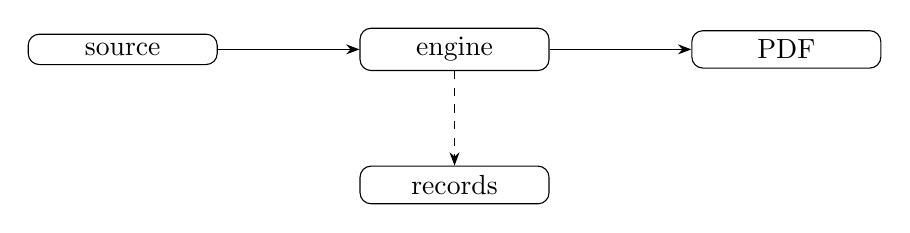
\begin{tikzpicture}[node distance=12mm and 18mm, every node/.style={draw, rounded corners, align=center, minimum width=24mm}]
    \node (src) {source};
    \node (eng) [right=of src] {engine};
    \node (pdf) [right=of eng] {PDF};
    \node (rec) [below=of eng] {records};
    \draw[-Stealth] (src) -- (eng);
    \draw[-Stealth] (eng) -- (pdf);
    \draw[-Stealth, dashed] (eng) -- (rec);
  \end{tikzpicture}
  \caption{One build, three artifacts.}\label{fig:pipeline}
\end{figure}

\section{Results}\label{sec:results}
\lipsum[8-10]
\Cref{tab:results} lists the measured phases; \cref{fig:plot} plots them, and
\cref{fig:example} is an included graphic \parencite{tantau:tikz,feuersaenger:pgfplots}.

\begin{table}[htbp]
  \centering
  \caption{Phases of a run.}\label{tab:results}
  \begin{tabular}{l S[table-format=3.1] S[table-format=2.1]}
    \toprule
    Phase & {Time (\si{\milli\second})} & {Share (\si{\percent})} \\
    \midrule
    startup & 120.0 & 30.0 \\
    preamble & 180.5 & 45.1 \\
    typesetting & 60.2 & 15.0 \\
    shipout & 20.1 & 5.0 \\
    finalization & 19.6 & 4.9 \\
    \bottomrule
  \end{tabular}
\end{table}

\begin{figure}[htbp]
  \centering
  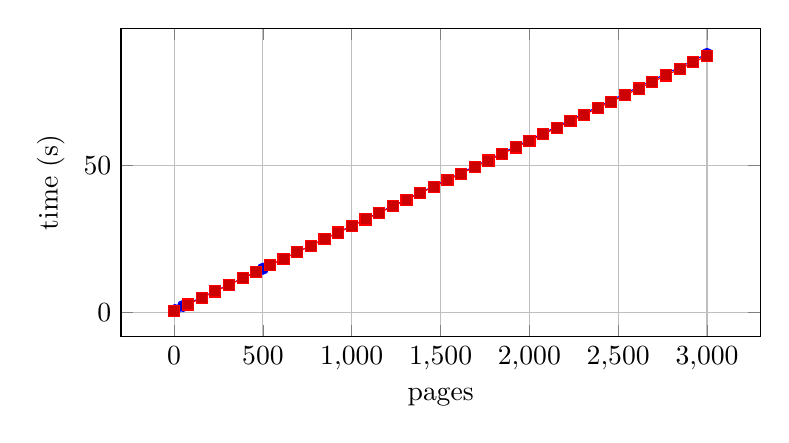
\begin{tikzpicture}
    \begin{axis}[width=0.8\linewidth, height=55mm, xlabel={pages}, ylabel={time (s)}, grid=major]
      \addplot+[mark=*] coordinates {(1,0.4) (5,0.7) (50,2.1) (500,14.8) (3000,88.0)};
      \addplot+[mark=square*, domain=1:3000, samples=40] {0.35 + 0.029*x};
    \end{axis}
  \end{tikzpicture}
  \caption{Time against pages.}\label{fig:plot}
\end{figure}

\begin{figure}[htbp]
  \centering
  \includegraphics[width=0.45\linewidth]{example-image-a}
  \caption{An included graphic.}\label{fig:example}
\end{figure}

\lipsum[11-14]

\section{Discussion}\label{sec:discussion}
\lipsum[15-18]
Related measurements are in \textcite{eijkhout:tex,mittelbach:hooks}, and the font
pipeline is described by \textcite{hagen:luatex,kew:xetex}.

\section{Conclusion}
\lipsum[19-21]
See \cref{sec:intro,sec:method,sec:results,sec:discussion} and \cref{fig:pipeline,tab:results}.

\printbibliography
\end{document}
